\documentclass{article}


\usepackage{arxiv}

\usepackage[utf8]{inputenc} % allow utf-8 input
\usepackage[T1]{fontenc}    % use 8-bit T1 fonts
\usepackage{hyperref}       % hyperlinks
\usepackage{url}            % simple URL typesetting
\usepackage{booktabs}       % professional-quality tables
\usepackage{amsfonts}       % blackboard math symbols
\usepackage{nicefrac}       % compact symbols for 1/2, etc.
\usepackage{microtype}      % microtypography
\usepackage{multirow}
\usepackage{multicol}
\usepackage{graphicx}
%\usepackage{natbib}
\usepackage[numbers,sort&compress]{natbib}
\usepackage{hyperref}
\usepackage{amsmath}
\usepackage{amssymb}
\usepackage{mathtools, nccmath}
%\usepackage{subcaption}
\usepackage{float}
\DeclarePairedDelimiter{\nint}\lfloor\rceil
\usepackage[linesnumbered,ruled,vlined]{algorithm2e}
%%%%%%%%%%% Defining Enunciations  %%%%%%%%%%%
\newtheorem{theorem}{\bf Theorem}[section]
\newtheorem{condition}{\bf Condition}[section]
\newtheorem{corollary}{\bf Corollary}[section]
%%%%%%%%%%%%%%%%%%%%%%%%%%%%%%%%%%%%%%%%%%%%%%%


\title{Dealing with uncertainty in agent-based models for short-term predictions}


\author{
  Le-Minh Kieu\thanks{Corresponding author} \\
  School of Geography \& Leeds Institute of Data Analytics\\
  University of Leeds\\
  United Kingdom \\
  \texttt{m.l.kieu@leeds.ac.uk} \\
  %% examples of more authors
   \And
 Nicolas Malleson \\
  School of Geography\\
  University of Leeds and Alan Turing Institute\\
  United Kingdom \\
  \texttt{n.s.malleson@leeds.ac.uk} \\
  \And
 Alison Heppenstall \\
  School of Geography\\
  University of Leeds and Alan Turing Institute\\
  United Kingdom \\
  \texttt{a.j.heppenstall@leeds.ac.uk} \\
}

\begin{document}
\maketitle

\begin{abstract}
Agent-based models (ABM) are gaining traction as one of the most powerful modelling tools within the social sciences.
They are particularly suited to simulating complex systems. Despite many methodological advances within ABM, one of the major drawbacks is their inability to 
incorporate real-time data to make accurate short-term predictions. This paper presents an approach that allows ABMs to be dynamically optimised. Through a combination of parameter calibration and data assimilation (DA), the accuracy of model-based predictions using ABM in real time is increased.  We use the exemplar of a bus route system to explore these methods.  
%Within this paper we construct an ABM that simulates the main interactions and key processes within this system. We develop an numerical experiment to quantify the impacts of calibration and DA in dealing the with stochastic and dynamic nature of the system under study. 
The bus route ABMs developed in this research are examples of ABMs that can be dynamically optimised by a combination of parameter calibration and DA. The proposed model and framework can also be used in an passenger information system, or in an Intelligent Transport Systems to provide forecasts of bus locations and arrival times. 
\end{abstract}


% keywords can be removed
\keywords{First keyword \and Second keyword \and More}


\section{Introduction} 
\label{s:Intro}

Agent-based modelling (ABM) \citep{bonabeau_agent_2002} is a field that excels in its ability to simulate
complex systems. Instead of deriving aggregated equations of system
dynamics, ABM encapsulates system-wide characteristics from the
behaviours and interactions of individual agents e.g. human, animals
or vehicles. ABM has emerged as an important tool for many 
applications ranging from urban traffic simulation
\citep{balmer2009matsim}, humanitarian assistance
\citep{crooks_gis_2013} to emergency evacuations
\citep{schoenharl_design_2011}.

Despite the many advances and applications of ABM, the field suffers from a serious drawback: models are currently  unable to incorporate up-to-date data to make accurate real-time predictions \citep{lloyd_exploring_2016, wang_data_2015,
ward_dynamic_2016}. Models are typically calibrated once, using historical data, then projected forward in time to make a prediction. Here, calibration is ideal for one point in time, but as the simulation progresses, the prediction rapidly diverges from reality  due to underlying uncertainties \citep{ward_dynamic_2016}. These uncertainties come from \textit{dynamic} (changing over space and time), \textit{stochastic} (containing inherent randomness) and \textit{unobserved} (unseen from the data) conditions of the real system under study. An example of such a system can be found in bus routes. Each time a bus reaches a bus stop, the number of alighting passengers is uncertain and the number of waiting passengers downstream is unobserved. The bus route's conditions also change over time, e.g. traffic varies over the route and with at off-peak to peak periods. 
%\end{fmtext}
There are methods to incorporate streaming data into models,
such as \textit{data assimilation} (DA) routines
\citep{lewis_dynamic_2006, wang2000data}. Broadly, DA refers to a suite of techniques that allow
observational data to be incorporated into models
\citep{wang2000data} to provide an optimal estimate of the
evolving state of the system. Performing DA increases the
probability of having an accurate representation of the current state of
the system, thereby reducing the uncertainty of future predictions. This is a technique that has been widely applied
in fields such as meteorology, hydrology and oceanography \citep{kalnay_atmospheric_2003}.

There are, however, two methodological challenges that must be overcome to apply DA in ABM. First, DA methods are often intrinsic to their underlying models which are typically systems of partial differential equations with functions linearised mathematically.  Hence DA methods typically rely on linearising the underlying model \citep{harvey1990forecasting}. One of the most appealing aspects of agent-based models is that they are inherently non-linear, so it is not clear whether the assumptions of traditional DA methods will hold. Second, it is still unknown how much uncertainty DA can effectively deal with when implemented within ABM. Assimilation of real-time data into ABMs has only been attempted a few times and these examples are limited by their simplicity \citep{lloyd_exploring_2016, wang_data_2015,
ward_dynamic_2016}.

This paper is part of a wider programme of work\footnote{\url{http://dust.leeds.ac.uk/}} that is focused on developing DA methods to be readily used in ABM. This paper focuses on one particular model that aims  to make predictions of bus locations in real time. Bus route operation has been chosen due to its inherent uncertainties -- for example a model will need to account for uncertain factors affecting how buses travel on the roads \citep{khosravi2011prediction} -- but also for its tractability -- there are many fewer interactions than present in, say, a model of a crowd.  We also focus on one particular DA algorithm -- the Particle Filter (PF). This method is chosen due to its ability to incorporate data into non-linear models such as ABMs \citep{carpenter1999improved}.

The objectives of this paper are to: (1) perform dynamic state estimation to reduce the
uncertainty in the model's estimate of the \textit{current} system state; (2) improve the accuracy of short term forecasts.

All the numerical experiments in this paper will be tightly controlled, following an `identical twin' experimental framework \citep[for example see][]{wang_data_2015}. We will first develop a complex ABM of a bus route to generate fine-grained synthetic GPS data of buses, that are reasonably similar to real GPS data, for use as synthetic `ground truth' data. We call this model the `BusSim-truth' model. The next step
is to develop companion ABMs that are of simpler nature than BusSim-truth that will not know the parameters of BusSim-truth and will not have the dynamic and stochastic features of BusSim-truth. We will calibrate and evaluate these companion ABMs against the data generated from BusSim-truth. This experiment is designed to be similar to the real-time monitoring and predictions of bus locations, where models are often a simpler version of reality, that are calibrated to be as close as possible to reality. The prediction of bus location and arrival times are essential for bus operators and a topical research challenge \citep{bin2006bus}. The methods developed here can easily be applied to simulation and forecasting for \textit{real} bus systems and could, therefore, offer considerable potential impact. This is particularly pertinent in rapidly developing cities where daily bus schedules can be extremely erratic. In these cases accurate, up-to-date estimates of current waiting times will be highly beneficial to citizens who use (or would like to use) public transport. 

The contributions of this paper are threefold. First, several ABMs of bus routes are constructed that account for the interactions between the bus and passengers, the bus and the surrounding traffic, and between multiple buses are considered. While model development is not the sole focus of this paper, these bus route ABMs are novel and have utility for other studies. Second, this paper introduces a combination of parameter calibration and DA techniques that can dynamically optimise an ABM to enable accurate estimation of the bus system in real time. Third, this paper shows and quantifies the impacts of calibration and DA in dealing the with stochastic and dynamic nature of the system under study.

This paper is structured as follows. Section~\ref{s:problem} describes
the research problem and the related works in the literature.
Section~\ref{s:method} outlines the methodology. Section~\ref{s:experiments} describes
the numerical experiments that are conducted and discusses these
results. Finally, Section~\ref{s:conclusion} concludes the study and
considers the opportunities for future work. 

% Other sections are in their own file

% !TEX root = BusSim.tex
% 
\section{Research problem and related works} \label{s:problem}

Historical and real-time bus GPS data is often used by operators to locate buses and predict their locations and arrival times. For instance, Public Transport Information and Priority System (PTIPS) is a state-of-the-art system in Australia to give priority to public transport vehicles on the roads and provide information on predicted bus arrival to passengers. The prediction of bus locations and arrival times in real time is a challenging problem \citep{chien2002dynamic}. Ideally, perfect 
knowledge of the current state of the system and any underlying processes is required.  However, obtaining this level of knowledge is impossible due to sources of uncertainty and the complex interactions in
bus operations. The majority of research within this area has focused on machine learning methods to find a direct mapping between input
data and bus arrival time. Examples of these methods include Artificial
Neural Networks \citep{chien2002dynamic}, Support Vector Machines
\citep{bin2006bus}, and Bayesian techniques
\citep{khosravi2011prediction}. While machine learning methods are generally
efficient in real time, they are solely reliant on the quality of available
data. Even with high-resolution datasets that record accurate spatio-temporal bus locations, the full complexity of the system will never be captured. 

%Without an understanding of the underlying processes driving bus operation, these models fail to quantify uncertainty and will perform poorly in highly stochastic systems, in unseen situations or when data are missing.

There are analytical and simulation models of bus routes that aim to
reproduce the underlying processes in bus operations, and shed some
light on the associated uncertainties. One of the earliest successes in simulating a simple bus systems was from Cellular Automata modelling
\citep{luo2012realistic,o1998jamming,chowdhury2000steady,
jiang2003realistic}. Whilst the dynamical foundations of these models
are well understood, they are outperformed by more sophisticated
models such as bus-following models
\citep{nagatani2000kinetic,huijberts2002analysis,Tang2012,
nagatani2001bunching,hill2003numerical}; and traffic-following models
\citep{cats2010mesoscopic,toledo2010mesoscopic,hans2015real}.
Bus-following models aim to model the fundamental dynamics of a bus
route by modelling individual buses that follow each other (for example speeding up if the bus ahead is far away). Traffic-following models,
on the other hand, aim to model buses as a component of a transport
system with private and public transport, where their speeds are
affected by the traffic flow, traffic signals \citep{hans2015real} or
traffic density \citep{toledo2010mesoscopic}.

The majority of these models are \textit{static}, i.e. they only have parameters that are fixed over time. We can represent these static simulators 
with the equation $Y = f(X)$, where $f$ represents the simulator. A run of a simulation is defined
as the process of producing one set of data $Y$ for a single set of
model parameters $X$. One way for these
models to reduce their uncertainty and fit more closely to the observed data is to
adjust the model parameters until the model satisfies some predetermined
criteria. This parameter adjustment process is often referred to as
\textit{parameter calibration}. Popular optimisation techniques include simulated annealing~\citep{pennisi_optimal_2008}, genetic
algorithms,~\citep{heppenstall_genetic_2007, malleson_optimising_2014},
and approximate Bayesian computation~\citep{grazzini_bayesian_2017}.
Parameter calibration, especially with ABMs, is often only
implemented once, and therefore cannot account for any changes that may take place within
the system. In the traffic context these might include accidents, traffic signal failures, vehicle faults, etc. Static models are simple to implement, but struggle to model dynamic systems. 


%Many advanced simulators are now \textit{dynamic}: they have inputs and
%outputs that vary over time and operate iteratively over fixed
%time steps. A real bus route is an example of a dynamic system, where
%the arrival rate of passengers and the surrounding traffic vary across
%different times of day, days of the week, and even seasonally. A dynamic
%simulator may be written in the form $Y_t = f(X_t)$, where $Y_t$ is the
%set of outputs at time $t$ and $X_t$ subsumes both fixed model
%parameters and time-varying variables at time step $t$. 

In real-time applications, e.g bus location or bus arrival time prediction in real time, prediction models often have to deal with the fact that there are so much uncertainty in bus operations. Real bus operation is \textit{dynamic} (changing over time) and also \textit{stochastic} (contains inherent randomness). In real time, there are also many unobservable information of bus operation, such as the number of passengers who are waiting at
downstream stops or the number who plan to get off the bus, and the
surrounding traffic conditions.  The lack of information about these factors means that any model of bus
operation in real time will have to make assumptions thereby introducing uncertainties. 

Therefore, this research will explore a combination of parameter calibration and a \textit{data
assimilation} (DA) technique to calibrate a dynamic ABM bus route simulator using historical data, and then dynamically optimised it on-the-fly using real-time data. This, in itself, is a novel and important
contribution. Few previous efforts have attempted to incorporate data
assimilation with agent-based models \citep[for example
see][]{ward_dynamic_2016, wang_data_2015}, and it is unclear how DA
methods, that have typically been created for linear models
\citep{harvey1990forecasting}, can be adapted for non-linear ABMs. 

DA methods assume that observational data are sparse and only describe
the target system in limited detail. Therefore a model is essential as a
means of filling in the gaps in space and time left by the observations through the generation of additional data.
In effect, the model propagates data from observed to unobserved areas
\citep{carrassi_data_2018}.  Although techniques can be used to
perform parameter estimation, they are most often framed as a state
estimation problem. The aim is to calculate a posterior probability for
the state vector $X_t$, given prior distributions from a model (in this
case, a bus route operation model) and data from observations. It is
this marriage of a model and real-time observational data (and the 
associated uncertainties) that offers the means of allowing all the
available information to be used to determine the true state of the
system as accurately as possible \citep{talagrand_use_1991}.

Models where the system state at time $t$ are only dependent on the state at time $t-1$ are termed \textit{Markovian}. We are particularly interested in ABMs that can be written in a Markovian nature because DA algorithms require knowledge to the \textit{full} model state in the form of the state vector $X_t$. While some ABMs in the literature track agent histories and use this information to decide future states, these can be recast as Markovian ABMs by expanding the state vector to include these histories. Implementing a bus route system as a Markovian model requires variables such as vehicle locations, speeds, occupancies etc. It is reasonable to
assume that the system state at the next time step only depends on the
value of these variables at the current time step. For simplicity, we
assume that the state vector used here has a fixed size.  The unused variables (i.e. those for buses that have yet to enter the system) can be set to zero, enabling the state vector to be treated as sparse and
passed efficiently between iterations. If the state vector has a fixed
size, then all possible states of the system belongs to a state-space
$\mathcal{X} \in \mathbb{R}^n$. The system state evolves in some fixed
interval \{0,..,K\}. We denote the state of the bus route at time $t$ by
$X_t \in \mathcal{X}$.

This paper follows an `identical twin' experiment framework \cite{wang_data_2015}, where experiment data to be used will be generated from simulation, instead of using real data. The reason is that real data often comes with noise that hides the true state of the bus route (e.g. noise from GPS data). A simulated synthetic data would enable us to control the level of noise in the data, and to evaluate the modelling results against the ground truth rather than noisy data. Figure \ref{fig:workflow} shows the workflow of this study. 

\begin{figure}[H]  \centering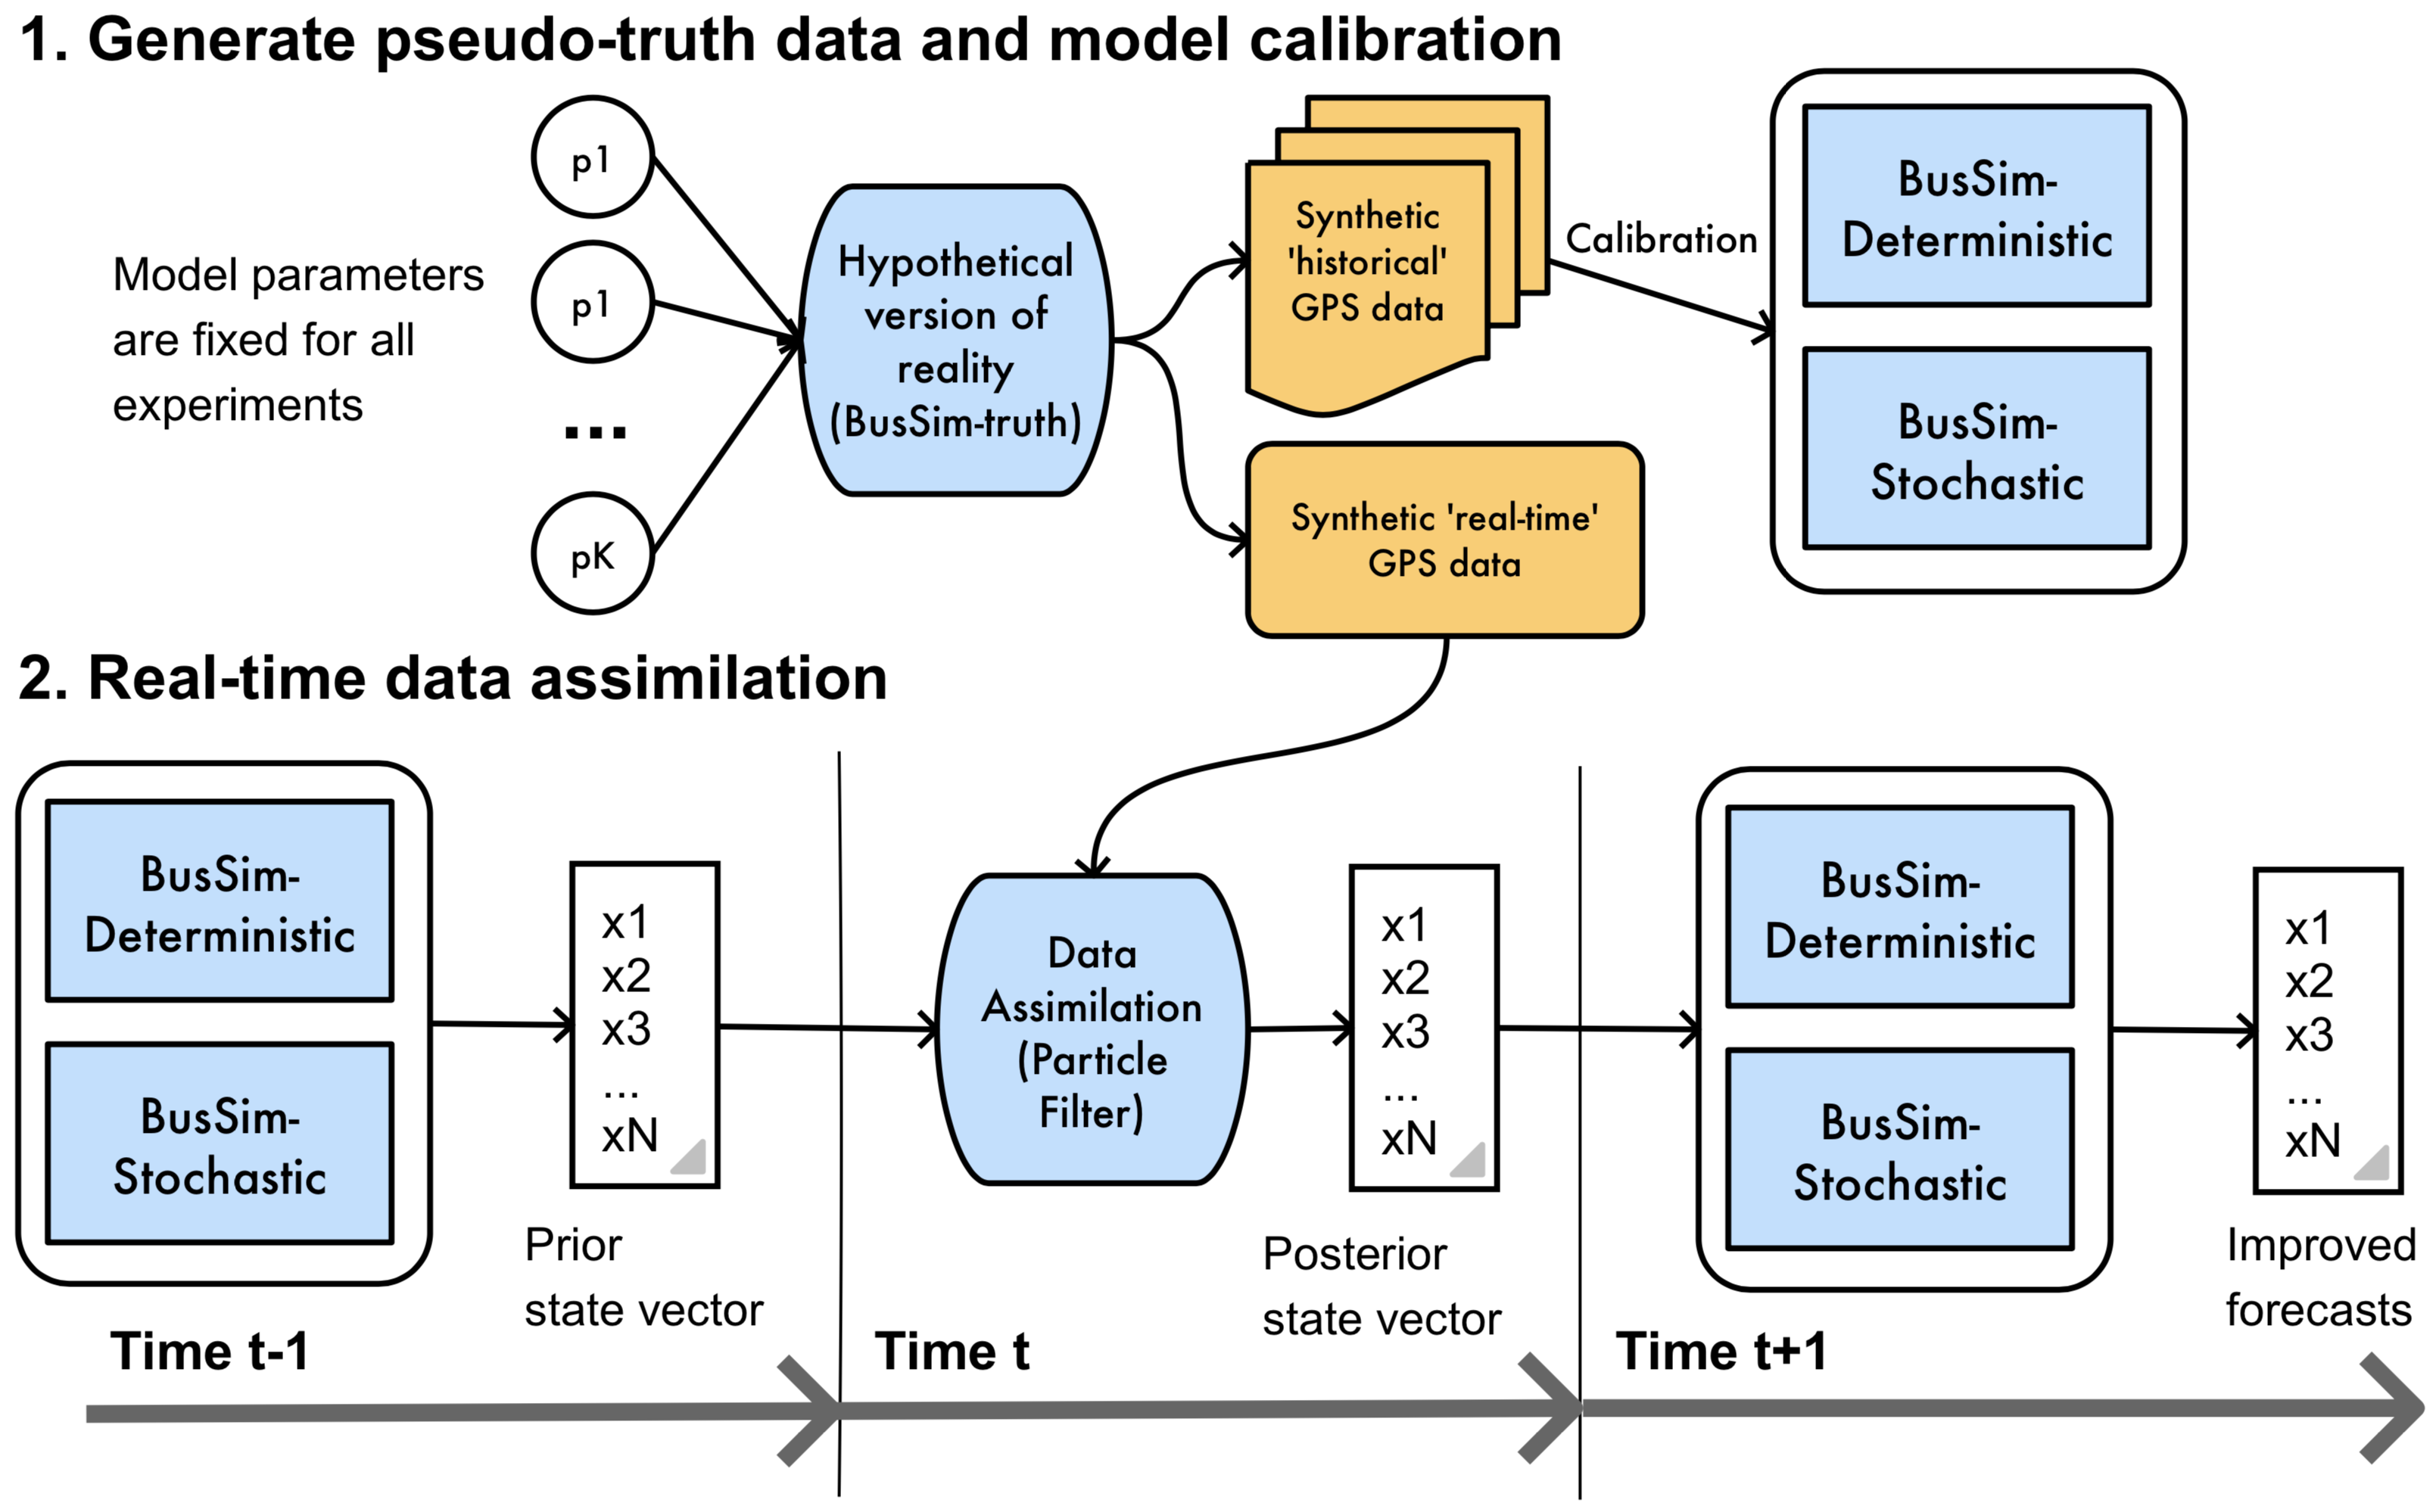
\includegraphics[width=13cm]{Figures/bussim-framework.png}
\caption{Study workflow.} 
\label{fig:workflow} 
\end{figure}

The study workflow generally consists of 2 major steps. It starts with the development of a Markovian ABM of bus route operation that will be referred as \textit{BusSim-truth}. BusSim-truth is a hypothetical version of reality and will be used to generate synthetic GPS data of bus locations with timestamps. Two sets of data will be generated. The first represents `historical' GPS data, which are essentially the outputs of multiple runs of the same BusSim-truth model with the same predefined set of parameters. The GPS data will be slightly different each time the model is run because BusSim-truth is stochastic (its outputs vary slightly from one run to another) and dynamic (the parameters that control factors such as the amount of traffic vary during a single model run). The second set of data represent a single run of BusSim-truth, also using the same set of parameters. These data will represent synthetic `real-time' GPS data and will be used to conduct data assimilation. This situation is similar to the reality, where `historical' data across multiple days are used to calibrate models and `real-time' data represent the \textit{current} state of the world. BusSim-truth will be reasonably realistic and will replicate popular phenomenon in bus operations such as bus bunching (two buses of the same line arrive at the same bus stop at the same time). 

In reality, any simulation model is a simplification of the actual dynamics. Taking this into consideration, we develop two simpler variations of BusSim-truth, knowing that they would not be able to perfectly represent the dynamics in BusSim-truth.  The two variations are: 
\begin{itemize} 
	\item \textbf{BusSim-deterministic}. This model evolves exactly the same way in each model run;
	\item \textbf{BusSim-stochastic}. This model is stochastic, e.g. the numbers of people waiting at bus stops is drawn from a random distribution 
\end{itemize} 

As would be necessary in reality, BusSim-deterministic and BusSim-stochastic will first be calibrated against the synthetic `historical' GPS data. In the second step of the study workflow, DA will be used in an attempt to update the states of the models to the `real-time' GPS observations in order to produce more accurate short-term forecasts of the system behaviour. 


% !TEX root = BusSim.tex
\section{Methodology\label{s:method}}

%\subsection{Notation}

%The following notation will be used to formalise each of the simulation models:
%\textbf{can the notation be put in the appendix as it takes up alot of room?}
%\label{s:Notation}
%\begin{itemize}
   % \item $dt$: Time interval ($s$)
    %\item $t$: Current time ($s$ from 00:00:00)
    %\item $N$: Number of buses
	%\item $j$: Index of vehicle $(j=1..N)$
%	\item $m$: Index of bus stop $(m=1..M)$
%	\item $M$: Number of bus stops
%	\item $c_j$: Current status of bus j (IDLE, MOVING, DWELLING or FINISHED). Where IDLE refers to out-of-service buses and DWELLING refers to buses that are serving passengers at stops. 
%	\item $a_j$: Acceleration rate of bus j ($m/s^2$)
%	\item $v_j$: Current speed of bus j ($m/s$)
%	\item $Occ_{j}$: Current occupancy of bus $j$ (number of passengers onboard)
%	\item $H$: Scheduled headway ($s$)
%	\item $C$: Bus capacity
%	\item $V$: Traffic speed ($m/s$)
%	\item $\delta_j$: The scheduled dispatch time of bus $j$ from the first stop
%	\item $t^a_{j,m}$: Arrival time of bus $j$ at stop $m$
%	\item $t^d_{j,m}$: The moment when bus $j$ can leave stop $m$ after passenger boarding and alighting (or $Leave\_stop\_time$)
   % \item $D_{j,m}$: Dwell time of bus $j$ at stop $m$ for passenger boarding and alighting
%	\item $\theta_1,\theta_2,\theta_3$: Parameters set for estimating $D_{j,m}$
%	\item $B_{j,m}$: Number of boarding passenger to bus $j$ at stop $m$
%	\item $A_{j,m}$: Number of alighting passenger from bus $j$ at stop $m$
%	\item $Arr_m$: Arrival rate of passengers to stop $m$ per second
%	\item $Dep_m$: Departure rate of passengers from stop $m$
%\end{itemize}

\subsection{A hypothetical version of reality: BusSim-truth and its two simpler variations}


The first step in the proposed workflow is to develop an agent-based bus route model that will be used to generate synthetic GPS data for each bus on the route (BusSim-truth). BusSim-truth is a stochastic and dynamic model with two classes of agents (bus and bus stop) and predefined parameters (see Table \ref{tab:Agents} ). It is stochastic because the number of boarding passengers is drawn from a random distribution, and dynamic because it parameters gradually change over time. The level of stochasticity and dynamicity in BusSim-truth can also be adjusted to represent bus route systems where conditions are largely stable or volatile over time.  

Figure \ref{fig:BusSim_flowchart} illustrates the workflow for BusSim-truth. Only a brief explanation of the model is included here, as more information on how the BusSim-truth model works can be found in the Appendix A. 
At each current time step, each Bus agent checks whether the next time step would be larger than the vehicle's scheduled dispatch time. If it is, we then check whether the bus is on the road (Status equals $MOVING$), or at a stop for passenger dwelling (Status equals $DWELLING$), or has finished its service (Status equals $FINISHED$), otherwise the bus remains $IDLE$.  

If the status is $MOVING$, we first check whether the bus is at a bus stop, by comparing the $GeoFence$ area of each bus stop agent with the bus' location. If the bus is not approaching a bus stop, its current speed will be compared with the surrounding traffic speed. In the case it is slower, we assume that the bus will speed up. If the speed already matches the traffic speed, the bus will maintain the same speed. Currently the traffic volume on the whole network is represented as a single dynamic parameter, although in practice it would be relatively trivial to make the traffic volume heterogeneous across the network. The system will first check if the stop is at the last stop when the bus is approaching a bus stop, where the bus' status will be changed to $FINISHED$ and the bus speed changed to zero. If it is not the last stop, the system will change the status of agent Bus to $DWELLING$ and its speed to zero. 
%Full details of how BusSim-truth works can be found in the Appendix.

\begin{table}[htbp]
  \centering
  \caption{Type of agents and their parameters in BusSim-truth}
    \resizebox{\textwidth}{!}{\begin{tabular}{ll}
    %\toprule
    \textbf{Parameter} & \textbf{Description} \\
    \midrule
     BusID  & Unique ID of the bus agent \\
          Acceleration & The acceleration value in $m/s^2$ if the bus needs to accelerate \\
           StoppingTime & Deadtime due to door opening and closing if the bus has to stop \\
           Visited & List of visited bus stops \\
           States & Whether the bus is idle, moving, dwelling or finished \\
           Trajectory & GPS coordinates of bus locations \\
    \midrule
    bus stopID & Unique ID of the bus stop \\
           Position & Distance from the first stop \\
           $Arr_m$ & Passengers arrived to the stop per second \\
           $Dep_m$ & Percentage of onboard passengers alight at the stop \\
           Arrival\_time & Store actual arrival time of buses at the stop \\
           GeoFence & A circle area to identify whether the bus is at the bus stop \\
    \bottomrule
    \end{tabular}}%
  \label{tab:Agents}%
\end{table}%

\begin{figure}[ht]
    \centering
    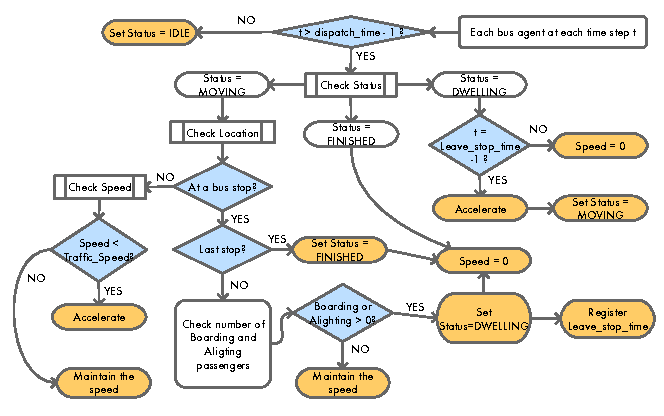
\includegraphics[width=1\textwidth]{Figures/flowchart.pdf}
    \caption{Flowchart of BusSim-truth.}
    \label{fig:BusSim_flowchart}
\end{figure}

As described in Section \ref{s:problem}, we use BusSim-truth to generate two sets of synthetic data: (1) `historical' GPS data that simulate normal bus route operation over a number of days and are used for calibration; and (2) `real-time' GPS data that represents a single run of the model and are used to represent the bus system \textit{today}. These are visualised in Figure~\ref{fig:historical_realtime}. Each record in the synthetic data is called an \textit{observation vector}. The vector contains all of the observations made from the `real world' (in this case the BusSim-truth).

\begin{figure}[h]
	\centering
	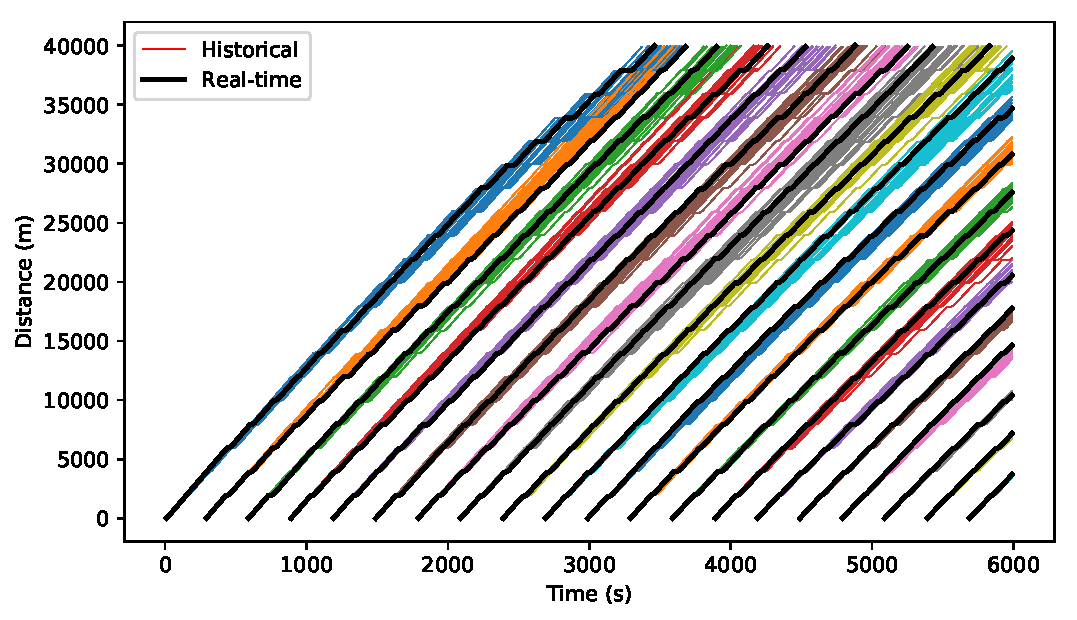
\includegraphics[width=1\textwidth]{Figures/Fig_spacetime_dynamic.pdf}
	\caption{Synthetic `historical' versus `real-time' GPS bus location data. Each coloured line shows the trajectory of one bus in the `historical' GPS data. As the BusSim-truth model is stochastic, there are differences between the trajectories. This is similar to the reality where buses operate slightly differently on multiple days. The bold black lines are another instance of bus trajectory that we consider as the `real-time' GPS data.  }
	\label{fig:historical_realtime}
\end{figure}

%\end{enumerate}

\subsection{Optimising the parameters of BusSim-deterministic and BusSim-stochastic}
\label{s:calibration}

Most agent-based models have a large number of parameters. For the BusSim models, the model parameter vector $S_t$ at time $t$ contains the arrival rate $Arr_m^t$, departure rate $Dep_m^t$ at each stop $m$, and the traffic speed $V^t$. 
\begin{equation}
  S_t  = \left[ \begin{array}{ccc}
Arr_m^t & Dep_m^t & V^t  
\end{array} \right] \quad m=1..M 
\label{eq:S}
\end{equation} 

The two simpler models (BusSim-deterministic and BusSim-stochastic) first need to be calibrated to the observations (the historical data). Here an automatic parameter calibration process, based on the Cross-Entropy Method (CEM) \citep{rubinstein1999cross} is used. CEM is a population-based Monte Carlo learning algorithm to combinatorial multi-extremal optimisation and importance sampling. It originated from the field of rare event simulation, where even small probabilities need to be estimated \citep{rubinstein1999cross}. In principle, CEM develops a \textit{probability distribution} over possible solutions for the optimal parameters of the model. New solution candidates are drawn from this distribution and are evaluated. The best candidates are then selected to form a new improved probability distribution of the optimal parameters, until certain criteria are met. CEM is chosen over some other popular optimisation methods in parameter calibration of ABMs, such as Genetic Algorithm \citep{heppenstall_genetic_2007} and simulated annealing~\citep{pennisi_optimal_2008}, because of its probabilistic nature that facilitates the calibration of stochastic models \citep{ngoduy2012calibration}. The interested reader may refer to \citep{rubinstein1999cross}, and various applications of CEM, such as \citep{ngoduy2012calibration}, for a more detailed account. A pseudo-code of the CEM algorithm that we adopted for this paper has also been described in Appendix B. 

Formally, the parameter calibration is an optimisation problem to minimise some performance index $PI(\pi)$ over all $\pi \in \mathbb{R}^k$. Here a solution $\pi= (\pi_1,\pi_2,...,\pi_k)$ denotes a set of parameters of the model under consideration and $k$ denotes the number of dimension in this set. Let $\pi_*$ denote the optimal solution, or the best set of model parameters that we want to find, that is:

\begin{equation}
    \pi_* = \text{argmin} \quad PI(\pi), \quad \pi \in \mathbb{R}^n
\end{equation}

The above objective function is equivalent to finding $\pi_*$ such that $PI(\pi_*) \leq PI(\pi) \quad \forall X \in \Pi$, where $\Pi$ is a constrained parameter space such that $\Pi \in \mathbb{R}^k$. The performance index $PI(\pi)$ is generally the difference between model output and observed data. The complexity of this problem comes from the stochasticity of BusSim, where the same solution $\pi$ may yield a different realisation $PI(\pi)$. To reduce this stochastic effect, it is necessary to run the (stochastic) model multiple times, and to evaluate the simulation outputs against a compilation of observed data from multiple days or instances. Let $K_I$ be the number of replications required for each model evaluation and $K_O$ be the number of instances in the observed data, we can derive a more detailed objective function of the parameter calibration problem: 

\begin{align}
    \text{min} \ PI(\pi) = \frac{1}{N \cdot T} \sum_{t=1}^T \sum_{n=1}^N \Bigg[ \bigg|  \frac{1}{K_I} \sum^{K_I}  s_{j,i,t}^{SIM}  - \frac{1}{K_O} \sum^{K_O}  s_{j,o,t}^{OBS} \bigg| + \nonumber \\
    \bigg| \sqrt{\frac{\sum^{K_I} \big( s_{j,i,t}^{SIM} - \hat{s}_{j,i,t}^{SIM} \big)^2}{K_I-1}}  - \sqrt{\frac{\sum^{K_O} \big( s_{j,o,t}^{OBS} - \hat{s}_{j,o,t}^{OBS} \big)^2}{K_O-1}} \bigg|   \Bigg]
    \label{eq:objective_function}
\end{align}

Where $N$ is the number of buses, $T$ is the number of time steps, $s_{j,i,t}^{SIM}$ is the location of simulated bus agent $j$ at time $t$ for the replication $i$, and similarly $s_{j,o,t}^{OBS}$ is the synthetic observed location of bus $j$ at time $t$ for the instance $o$. The objective function in Equation \ref{eq:objective_function} can be seen as the sum of the difference in mean location and standard deviation of locations at each time step for each bus and each replication/instance between simulated outputs and synthetic observed data. We want to evaluate the difference in not just the mean but also the standard deviation of bus locations because the system under study is stochastic, so it is not just the mean but also the spread of bus locations over multiple instances are important. 

\subsection{Data Assimilation using a Particle Filter (PF)}
\label{s:PF}

We can formulate an ABM as a state-space model $\dot{X}_t = f(X_{t}) + \epsilon_t$ and use data assimilation (DA) to dynamically optimise the model variables with up-to-date data to reduce uncertainty. The state-space model is represented by a state-space vector $X_t$ at time $t$, which contains all information of the current state of each agent in the model: 
\begin{align}
    X_t = \left[ O_t \quad S_t \right] \nonumber \\
    =\left[ \begin{array}{ccccccc}
c_j^t & s_j^t & v_j^t & Occ_j^t & Arr_m^t & Dep_m^t & V^t \end{array} \right] 
\label{eq:state_vector}
\end{align}
  
The state-space vector $X_t$ must contain all of the information that identifies the current state of the modelled system, allowing it to be projected forward to the next time step. Thus vector $X_t$ usually contains both the observation vector $O_t$ and the model parameters vector $S_t$ (Equation \ref{eq:S}) at time $t$. Note that $S_t$ has been calibrated in the previous section, but is still included in the state space vector $X_t$ to allow the model to be dynamically optimised with new data -- this is essential in dynamic situations where parameter values change over time. This approach is often referred to as dynamic calibration \citep{eicker2014calibration}.

Data Assimilation (DA) is a suite of methods to adjust the state of a running model using new data to better represent the current state of the system under study \citep{ward_dynamic_2016}. DA was born out of data scarcity, where observation data are sparse and insufficient to describe the system. Notwithstanding the proliferation of new data sources, insufficient data is still a major problem in research. The prediction of bus locations is a clear example where the number of future boarding and alighting passengers are unknown in real time. DA algorithms fill in the spatio-temporal gaps in the observed data by running a model forward in time until new observed data are available. This is typically called the \textit{predict} step in DA algorithms. After the predict step, DA has an estimate of the current system state and its uncertainty (which is often referred as the `prior' in Bayesian literature). The next step is typically called the \textit{update} step, where new observations and uncertainty are used to update the current state estimates. The result is referred to as the `posterior' in Bayesian literature, and should be the best guest of the system state from both the observations and model.

There are several DA algorithms in the literature, ranging from the simple Kalman Filter \citep{meinhold1983understanding} to more advanced extensions, including extended, ensemble and unscented Kalman Filter \citep{ward_dynamic_2016}. These algorithms generally aim to extend the original Kalman Filter by relaxing the assumption of linearity and introducing methods to work with non-linear models. However, they may not be the most suitable candidate to incorporate data into ABMs for two reasons. First, ABMs are driven by a large number of interacting agents with goals, history and behavioural rules. As a result, they lack an analytic structure, such as differential or difference equations, to facilitate the implementation of the Kalman Filter and its extensions where often the model Jacobian and covariance matrices need to be formulated \citep{wang_data_2015}. Second, although the assumption of linearity has been relaxed, these extensions assume that the noise in the model estimation is Gaussian. 

There is a flexible Bayesian filtering method that has been designed to work with non-linear, non-Gaussian models without analytical structure; this is the Particle Filter (PF). The key idea is to approximate a posterior distribution by a set of samples or particles, drawn from this distribution. Each particle is a concrete hypothesis of the true system state. The set of particles approximates the posterior distribution. PF is best described as a nonparametric Bayes filter because it develops the belief using a finite number of samples. 

Hypotheses of the system state at time $t$ is represented by a set $P_t$ of $N_P$ weighted random particles: 
\begin{equation} 
    P_t =  \{  \langle X_t^{\nint{i}}, w_t^{\nint{i}} \rangle \ | \ i=1,...,N_P \}
\label{eq:system_state_particle}
\end{equation}

where $X_t^{\nint{i}}$ is the state vector of the \textit{i}-th particle and $w_t^{\nint{i}}$ is the corresponding weight. Weights are non-zero, and sum over all weights is 1. The core idea of the PF is to update and maintain this set of particles given model outputs and observations. A PF recursively estimates the particle set $P_t$ based on the estimate $P_{t-1}$ at the previous time step, and the observation. The PF algorithm can be briefly described in three steps:
\begin{enumerate}
	
    \item \textbf{Predict:} Generate the next set of particles $\hat{P}_t$ from the previous set $P_{t-1}$. This represents the \textit{prior} distribution to describe how the system state evolves. 
    \item \textbf{Importance Weighting:} Compute the importance weight $w_t^{\nint{i}}$ for each particle in $P_t$. This is equivalent to the `Update' step in Kalman Filter, and will give us the \textit{posterior} distribution 
    \item \textbf{Resampling:} This step has no analogous step in Kalman Filter and its extensions. The resampling step creates a new set of particles from the current set. The likelihood to draw a particle is proportional to its weight. We adopt Sample Importance Resampling (SIR), a popular bootstrap systematic resampling in the PF literature \citep{wang_data_2015, carrassi_data_2018}. SIR has been developed to deal with \textit{particle deprivation}, which is the problem when particles converge to a single particle after several iterations due to one particle outperforming all others \citep{kong_sequential_1994}. This problem significantly reduces the area of state space covered by the particles in later iterations. 
\end{enumerate}
    Since resampling will generate particles using the existing pool of particles, it will not be able to produce particles where the prediction accuracy is better than the existing particle pool. This means that in \textit{classical} PF, the model parameter $S_t$ of both BusSim-deterministic and BusSim-stochastic will be unchanged over time. Because the  parameters change over time, we need to dynamically optimise $S_t$. This problem is solved in this paper by a simple and generic solution. We improve the quality of the particles by diversification similar to \citep{vadakkepat_improved_2006}, in a process also known as roughening, jittering, and diffusing \citep{pantrigo_combining_2005}. This is achieved by adding a random Gaussian white noise $\sigma$ with mean 0 and a predefined standard deviation, not to the whole state vector $X_t$, but to the model parameter $S_t$, to increase the probability of having particles that represent the current state of the underlying model. 
    
The PF is applied to BusSim-deterministic and BusSim-stochastic using up-to-date data from the synthetic `real-time' GPS data. 



% !TEX root = ParticleFilter.tex
\section{Experimental Results\label{experiments}}

\subsection{Outline of the Experiments}

Recall that the aim of the paper is to \aim. By examining the error (i.e. the difference between the particle filter estimate of the system state and the pseudo-truth data) under different conditions, the paper will present some preliminary estimates of the potential for the use of particle filtering in real-time crowd simulation. In particular, the paper will estimate the minimum number of particles ($N_p$) that are needed to model a system that has a given number of agents ($N_a$). Although the dynamics of the model used here are simpler than those of more advanced crowd models, and hence the particle filter is tasked with an easier problem than it would have to solve in a real-world scenario, these experiments provide valuable insight into the general \textit{potential} of the method for crowd simulation.

It is well known that one of the main drawbacks with a particle filter is that the number of particles required can explode as the complexity of the system increases~\citep[e.g.][]{snyder_obstacles_2008, carrassi_data_2018}. In this system, the complexity of the model is determined by the number of agents. As outlined in Section~\ref{method}, randomness is introduced through agent interactions.  Therefore the fewer the number of agents, the smaller the chance of interactions occurring and the lower the complexity. As the number of agents increases,we find that the number of interactions increases exponentially (Figure~\ref{fig:collision_count}, discussed in the following section, will illustrate this). The paper will also experiment with the amount of particle noise that needs to be included to reduce the problem of particle deprivation ($\sigma_p$), but this is not a focus of the experiments.

%Figure~\ref{fig:PF_flowchart} outlined the modelling process. The particle filter runs in parallel to a single instance of the StationSim model, which is used to create pseudo-truth data (observations) representing the the locations of each agent at a given iteration. In each data assimilation `window', the truth model and all particles are stepped forward a number of iterations. At the end of the window the particle filter receives pseudo-true observations and uses these to calculate the particle weights (i.e. the error associated with each particle).  

To quantify the `success' of each parameter configuration -- i.e. the number of particles $N_p$ and amount of particle noise $\sigma_p$ that allow the particle filter to reliably represent a system of $N_a$ agents -- an estimate of the overall error associated with a particular particle filter configuration is required. There are a number of different ways that this error could be calculated. Here, we calculate the mean weight of each particle after resampling in every data assimilation window (the weights vary during an experiment because in early windows there are few agents and hence very little stochasticity so particle errors are low). Then we take the mean of these individual particle errors. In addition, because the results from an individual experiment can vary slightly, each particle configuration is executed a number of times, $M$, and the median error across experiments is calculated.

Formally if $\nu(t,j)$ is the error of particle $j$ in a data assimilation window $t$, and the total number of windows is $T$, then the total error of that particle filter configuration across $M$  experiments is: 
\begin{equation}
  E_{N_p,\sigma_p,N_a} =  {\rm median}_M \left( \sum_{j=1}^{N_p}  \frac{\sum_{t=1}^{T}\nu(t)}{T} \right)
\end{equation}
where $median_M()$ calculates the median over $M$ experiments.

In summary, the Table~\ref{tab:experiment_parameters} outlines the parameters that are used in the experiments. There are a number of other model and particle filter parameters that can vary, but ultimately these do not influence the results outlined here and are not experimented with. The parameters, and code, are available in full from the project repository \cite{stationsimgit}. 
% \begin{quote}\url{XXXX github url}\end{quote}

\begin{table*}[ht] \caption{Main parameters used in the experiments}
	\begin{center}
		\begin{tabular}{l l l } 
		    \hline Parameter & Symbol & Value / Range \\
			\hline
			Number of agents & $N_a$ & $[ 2, 40 ]$ \\
			Number of particles & $N_p$ & $[ 1, 10000 ]$ \\
			Particle noise & $\sigma_p $ & $[0.25, 0.5]$ \\
			Measurement noise & $\sigma_m$ &  $1.0$ \\
			Number of experiments (repetitions) & M & 20 \\
			Model iterations in each data assimilation window & - & 100 \\ 
			\hline
	\end{tabular} \end{center} \label{tab:experiment_parameters}
\end{table*}%



\subsection{Results}

\subsubsection{Overall Error}

Figure~\ref{fig:median_abs_error} plots the median of the mean error over all experiments to show how it varies with differing numbers of agents and particles. Due to the computational difficulty in running experiments with large numbers of particles and the need for an exponential increase in the number of particles with the number of agents (discussed in detail below), there are fewer experiments with large numbers of particles and hence the the experiments are not distributed evenly across the agents/particles space. Thus the error is presented in the form of an interpolated heat map. Broadly there is a reduction in error from the bottom-right corner (few particles, many agents) to the top left corner (many particles, few agents). The results illustrate that, as expected, there is a larger error with increasing numbers of agents but this can be mediated with larger numbers of particles. Note the logarithmic scale used on the vertical axis; an exponentially greater number of particles is required for each additional agent included in the simulation. 

\begin{figure}[ht]
	\centering
	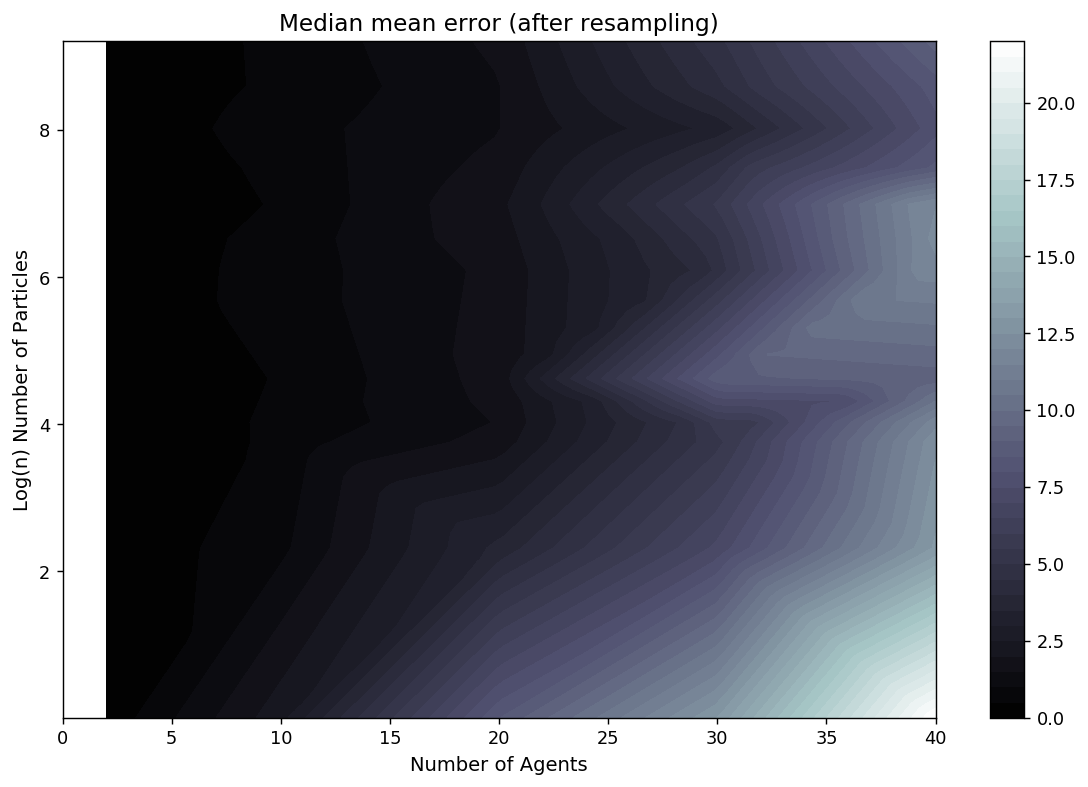
\includegraphics[width=0.7\textwidth]{figures/results/median_abs_error}
	\caption{Median of the mean errors after resampling} \label{fig:median_abs_error}
\end{figure}

There are two reasons for this exponential increase in the number of particles required. Firstly, as the number of agents increases so does the dimensionality of the state space. Also, and perhaps more importantly, with additional agents the chances of collisions, and hence stochastic behaviour, increases exponentially. This is illustrated by Figure~\ref{fig:collision_count} which presents the total number of collisions that occur across a number of simulations with a given number of agents.

\begin{figure}[ht]
	\centering
	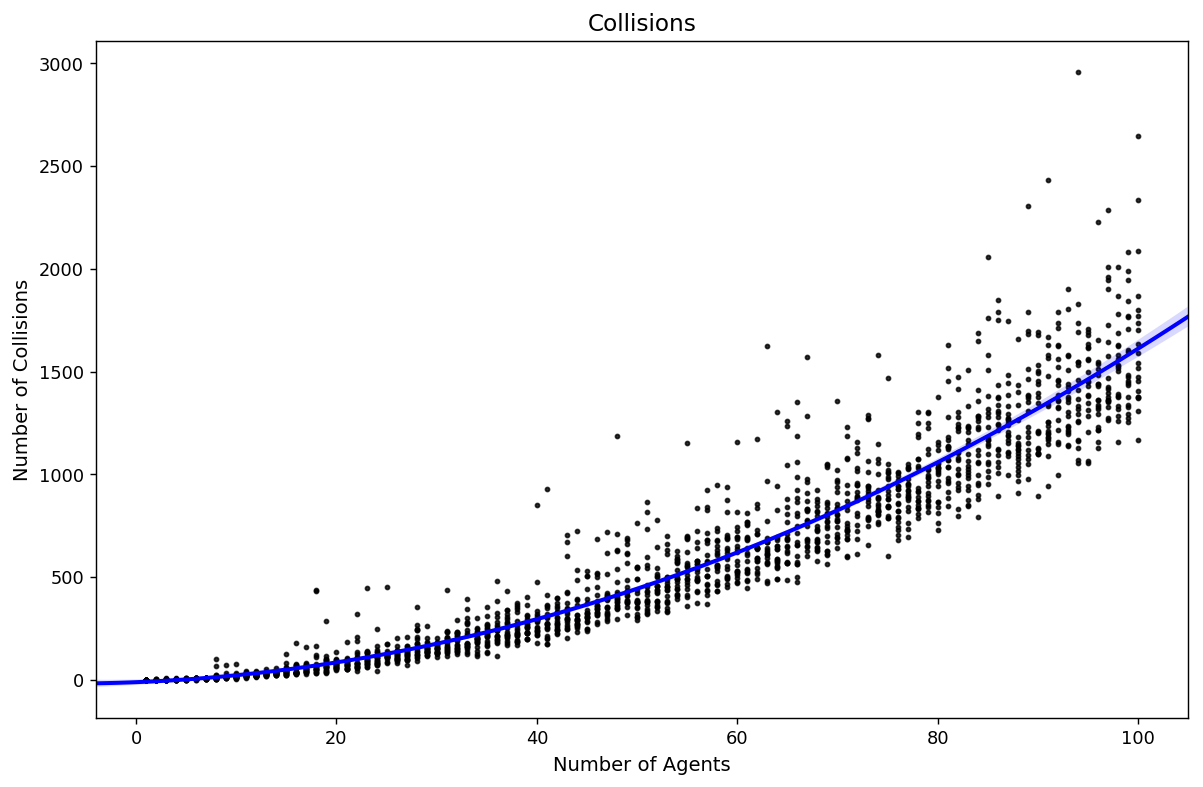
\includegraphics[width=0.7\textwidth]{figures/results/wiggle_count}
	\caption{The total number of collisions that occur given the number of agents. The blue line represents a polynomial regression model of order 2 with 99\% confidence intervals.} \label{fig:collision_count}
\end{figure}

On its own, the overall particle filter error (Figure~\ref{fig:median_abs_error}) reveals little information about which configurations would be judged `sufficiently reliable' to be used in practice. Therefore it is illuminating to visualise some of the results of individual particle filter runs to see how the estimates of the individual agents' locations vary, and what might be considered an `acceptable' estimate of the true state. Figure~\ref{fig:ani-10agents-10particles} illustrates the state of a particle filter with 10 particles and 10 agents at the end of its first data assimilation window (after resampling). With only ten agents in the system there are few, if any, collisions and hence very little stochasticity; all particles are able to represent the locations of the agents accurately.

\begin{figure}[ht]
	\centering
	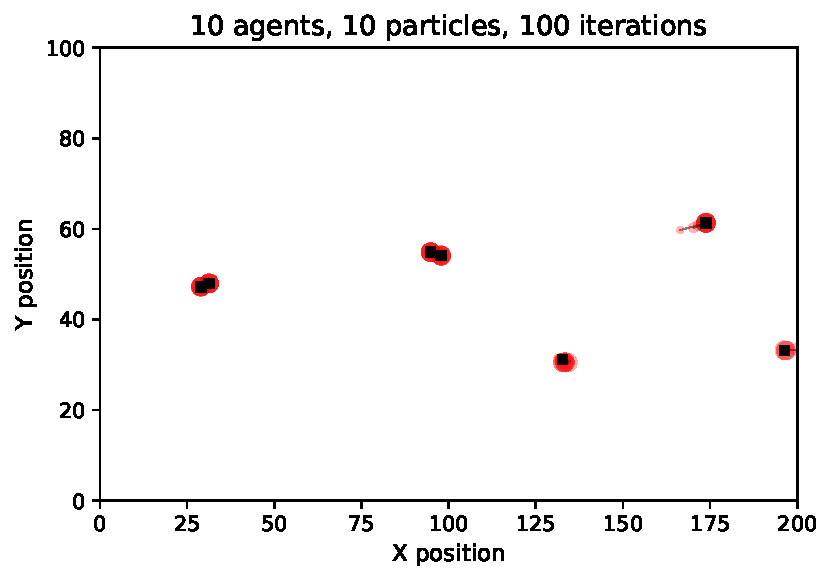
\includegraphics[width=0.45\textwidth]{figures/results/ani-10agents-10particles-window100}
	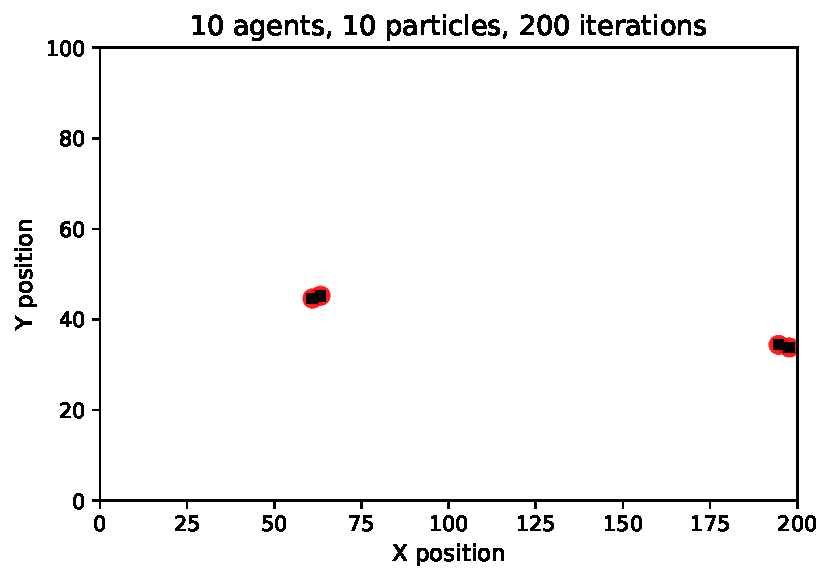
\includegraphics[width=0.45\textwidth]{figures/results/ani-10agents-10particles-window200}
	\caption{State of a particle filter with 10 agents and 10 particles after 100 and 200 iterations (after resampling at the end of the first and second data assimilation windows). Black squares illustrate the (pseudo) real locations of the agents and red circles represent the locations of those agents as predicted by individual particles (in this case all particles predict the agents' locations accurately and hence the red circles overlap).} \label{fig:ani-10agents-10particles}
\end{figure}

As the number of agents increases, collisions become much more likely and the chance of a particle diverging from the pseudo-truth state increases considerably. It becomes more common that no single particle will correctly capture the behaviours of \textit{all} agents. Therefore even after resampling there are some agents whose locations the particle filter is not able to accurately represent. Figure~\ref{fig:ani-50agents-10particles} illustrates a filter running with 40 agents and still only 10 particles. The long black lines show the locations of pseudo-real agents and the corresponding agents in the individual particles; it is clear that for some agents none of the particles have captured their pseudo-real locations. This problem can be mediated by increasing the number of particles. Figure~\ref{fig:median_abs_error} showed that with approximately 10,000 particles the error for simulations with 40 agents drops to levels that are comparable to the simulations of 10 agents. Hence a rule of thumb is that any particle filter with an overall error that is comparable to a clearly successful filter (i.e. Figure~\ref{fig:ani-10agents-10particles}) are reliably estimating the state of the system.

\begin{figure}[ht]
	\centering
	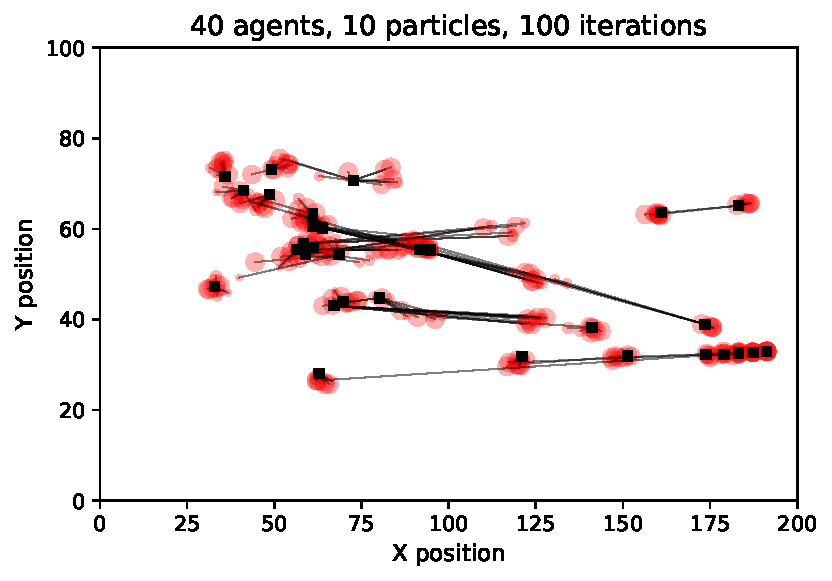
\includegraphics[width=0.45\textwidth]{figures/results/ani-40agents-10particles-window100}
	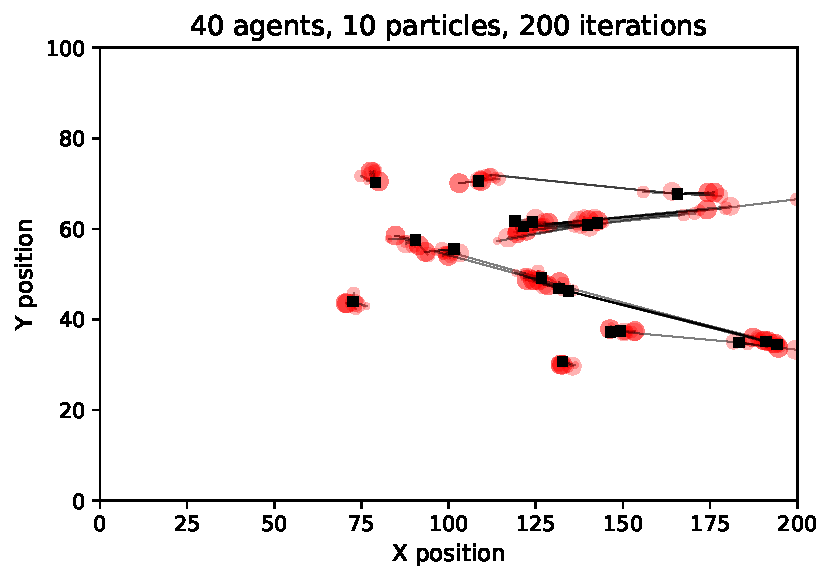
\includegraphics[width=0.45\textwidth]{figures/results/ani-40agents-10particles-window200}
	\caption{State of a particle filter with 50 agents and 10 particles. Lines connecting black squares (the pseudo-real agent locations) to red circles (particle estimate of the agent location) show that some particle estimates are a long way from the true agent locations.} \label{fig:ani-50agents-10particles}
\end{figure}



\subsubsection{Impact of Resampling}

Resampling is the process of weighting all particles according to how well they represent the pseudo-truth data; those with higher weights are more likely to be sampled and used in the following data assimilation window. This is important to analyse because it is the means by which the particle filter improves the overall quality of its estimates. Figure~\ref{fig:resampling} illustrates the impact of resampling on the error of the particle filter. With fewer than 10 agents in the system resampling is unnecessary because all particles are able to successfully model the state of the system. With more than 10 agents, however, it becomes clear that the population of particles will rapidly diverge from the pseudo-truth system state and resampling is essential for the filter manage to limit the overall error.

\begin{figure}[ht]
	\centering
	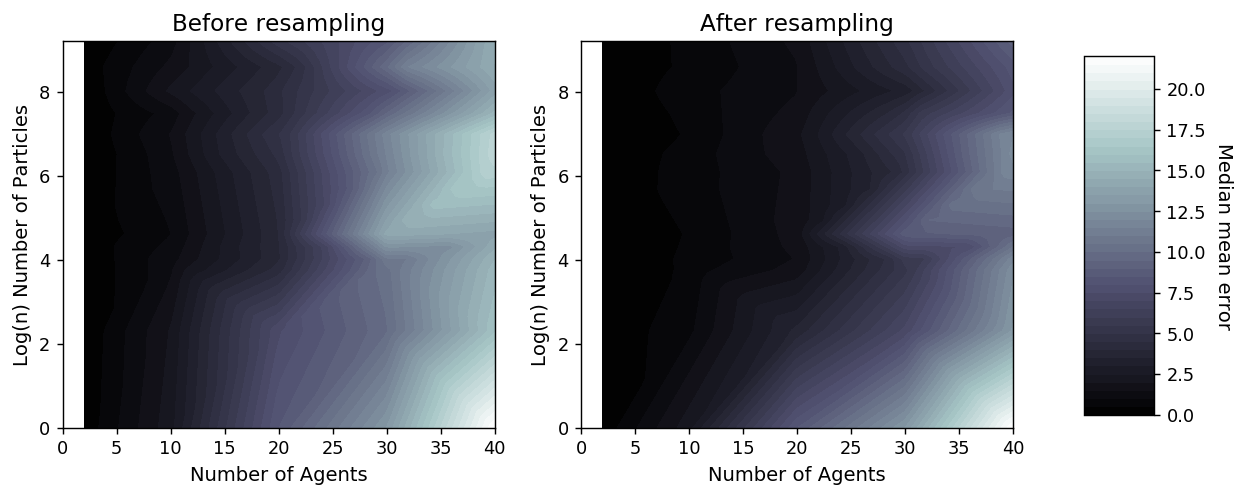
\includegraphics[width=0.9\textwidth]{figures/results/resampling}
	\caption{Median of the mean errors before and after resampling}\label{fig:resampling}
\end{figure}

\subsubsection{Particle Variance}

As discussed in Section~\ref{particle_sampling}, the variance of the population of particles can be a reliable measure for estimating whether particle deprivation is occurring. If there is very little variance in the particles, then it is likely that they have converged close to a single point in the space of possible states. This needs to be avoided because, in such situations, it is extremely unlikely that any particles will reliably represent the state of the real system. Figure~\ref{fig:variance_results} illustrates this by visualising the mean error of all particles, $\nu(t)$ (defined in Equation~\ref{eqn:particle_error}), in each data assimilation window, $t$, and their variance under different numbers of agents and particles. Note that each agent/particle configuration is executed 10 times and the results are visualised as boxplots. Also, simulations with larger numbers of agents are likely to run for a larger number of iterations, but the long-running models usually have very few agents in them in later iterations (most have left, leaving only a few slow agents). Hence only errors up to 600 iterations, where most of the agents have left the environment in most of the simulations, are shown. The graphs in Figure~\ref{fig:variance_results} can be interpreted as follows: 

\begin{figure}[ht]
	\centering
	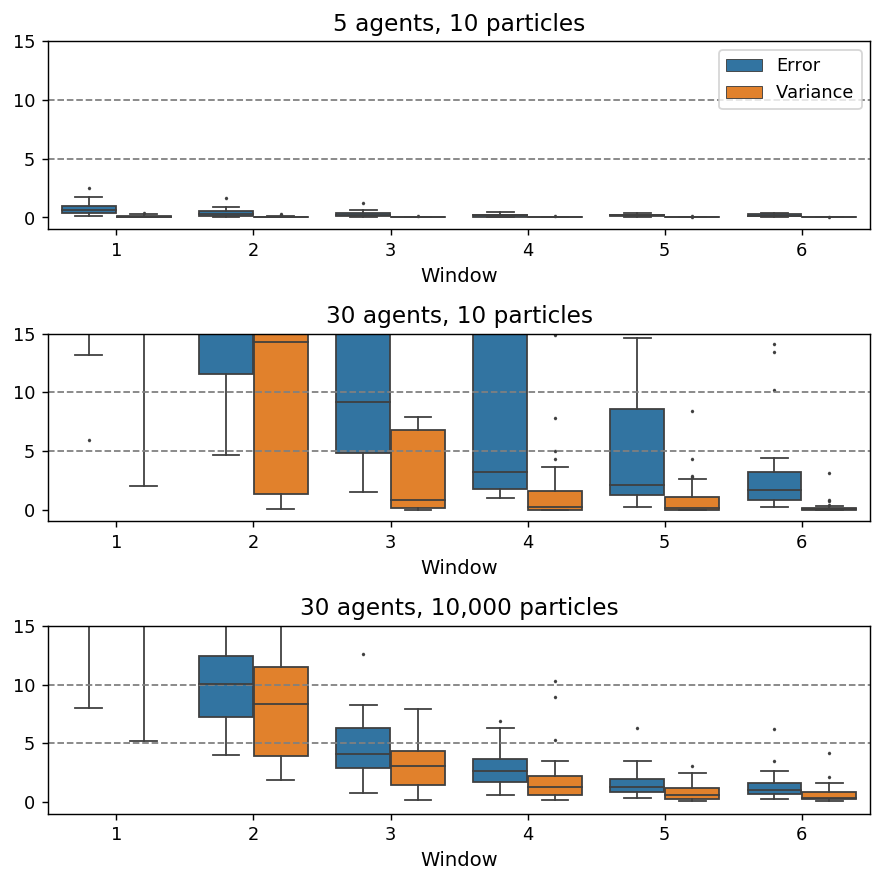
\includegraphics[width=0.9\textwidth]{figures/results/variance_results}
	\caption{Mean error and variance of particles under different combinations of the number of particles and number of agents}\label{fig:variance_results}
\end{figure}

\begin{itemize}
    \item With \textbf{5 agents and 10 particles} there is very low error and low variance (so low that the box plots are difficult to make out on Figure~\ref{fig:variance_results}). This suggests that particle deprivation is occurring, but there are so few agents that the simulation is largely deterministic so the particles are likely to simulate the pseudo-truth observations accurately regardless.
    \item When the number of agents is increased to \textbf{30 agents and 10 particles}, the errors are much larger. The increased non-linearity introduced by the greater number of agents (and hence greater number of collisions) means that the population of particles, as a whole, is not able to simulate the pseudo-truth data. Although particle variance can be high, none of the particles are successfully simulating the target.
    \item Finally, with \textbf{30 agents and 10,000 particles}, the errors are relatively low in comparison, especially after the first few data assimilation windows. 
\end{itemize}




\subsubsection{Particle Noise}

The number of particles ($N_p$) is the most important hyper-parameter, but the amount of noise added to the particles ($\sigma_p$) is also important as this is the means by which particle deprivation is prevented. However, the addition of too much noise will push a particle a long way away from the true underlying state. Under these circumstances, although particle deprivation is unlikely none of the particles will be close to the true state. To illustrate this, Figure~\ref{fig:median_abs_error-noise2.0} presents the median error with a greater amount of noise ($\sigma_p=0.5$). The overall pattern is similar to the equivalent graph produced with $\sigma_p=0.25$ in Figure~\ref{fig:median_abs_error} -- as the number of agents in the simulation ($N_a$) increases so does the number of particles required to maintain low error ($N_p$)  -- but the overall error in each $N_a$/$N_p$ combination is substantially larger for the experiments with additional noise. Future work could explore the optimal amount of noise in more detail; $\sigma=0.25$ was found to be the most reliable through trial and error.

\begin{figure}[ht]
	\centering
	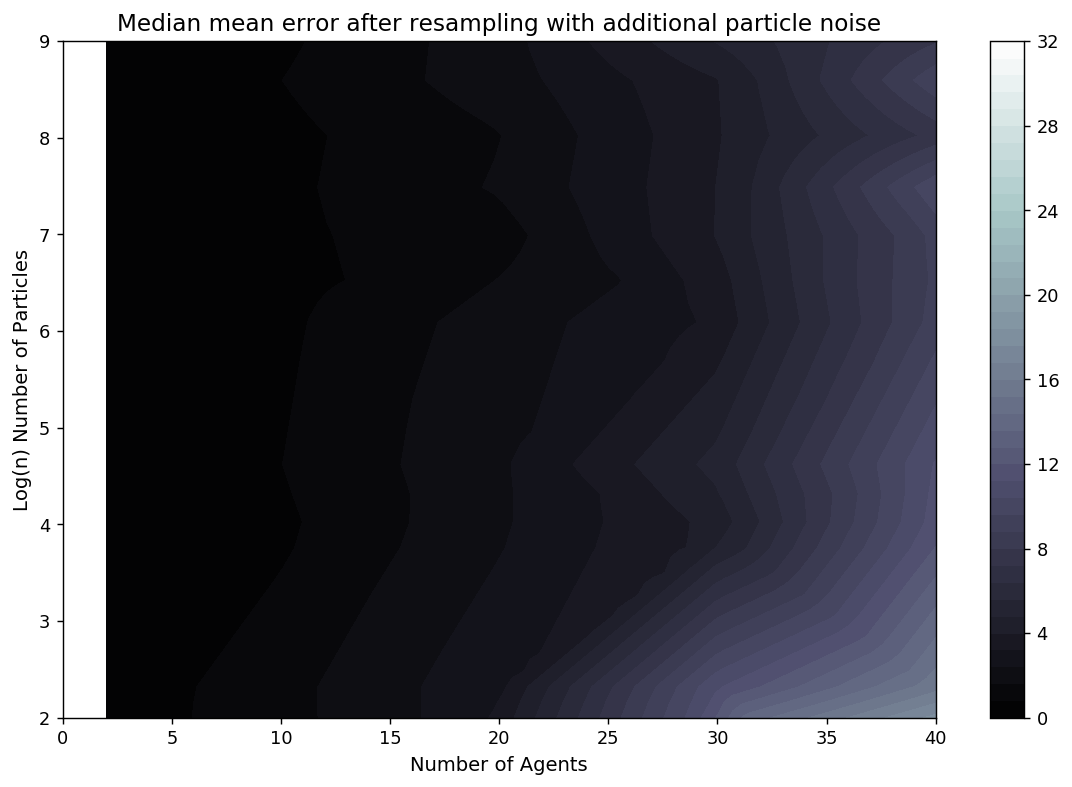
\includegraphics[width=0.5\textwidth]{figures/results/median_abs_error-noise2_0}
	\caption{Median of the mean errors after resampling with additional noise ($\sigma=0.5$).} \label{fig:median_abs_error-noise2.0}
\end{figure}



% !TEX root = BusSim.tex
\section{Implications\label{s:implications}}

This paper presents an integrated framework to reduce uncertainty in ABMs when making predictions in real time, by combining parameter calibration and data assimilation. As discussed in Section \ref{s:Intro} and \ref{s:problem}, an `identical twin' approach has been adopted instead of real noisy data to facilitate an effective evaluation of the proposed methods against the synthetic `ground truth'. The numerical experiment shows that the framework yields more accurate predictions than (i) a benchmark scenario (without parameter calibration), and (ii) a scenario with parameter calibration but without data assimilation. 

In its current form, the framework can provide \textit{real time} bus locations and arrival times for passenger information systems. The forecasted bus location and arrival information provides key intelligence for waiting passengers \cite{fan2016waiting}. This is beneficial for all public transport passengers, but can be of particular benefit in countries, for example in the Global South \cite{kumar2017bus} where  there are frequent delays due to transport systems being complex, heterogeneous or heavily congested. The prediction of bus arrival times is also critical for real-time trip planners. These planning systems propose optimal alternative routes for passengers, or update information on a connecting service that may be unreachable due to delayed buses. 

Many advanced Intelligent Transport System applications heavily rely on predictions of bus location and arrival times, for  example  bus control studies such as \cite{daganzo2009headway}.  A model-based prediction of bus location and arrival time, such as the framework in this paper, would allow bus operators the ability to evaluate and update their transportation infrastructures in real time.



% !TEX root = BusSim.tex
\section{Conclusion\label{s:conclusion}}

This paper proposes parameter calibration and data assimilation frameworks to enhance the prediction accuracy in agent-based models (ABM) when the system under study has a \textit{stochastic} and \textit{dynamic} nature. This is done in a 'identical twin' approach. We first develop a stochastic and dynamic ABM of bus route, referred to as \textit{BusSim-truth}. This model is employed to generate synthetic `historical' and `real-time' GPS data of bus locations. The `historical' data is used to train two simpler models of bus route, referred to as \textit{BusSim-deterministic} and \textit{BusSim-stochastic}, and evaluate against the 'real-time' data. 

Similar to the practice, when any simulation model is a simplification of the reality, BusSim-deterministic and BusSim-stochastic are simpler than BusSim-truth, and thus may not be able to produce a prediction similar to the synthetic `real-time' GPS data under limited data. We propose a solution for this issue by parameter calibration using Cross-Entropy Method (Scenario 2), by a combination of parameter calibration and Particle Filtering (Scenario 3), and show that they outperform the no calibration scenario (Scenario 1) and only Particle Filtering scenario (Scenario 4), at various levels of uncertainty. 

This paper shows the need for parameter calibration and data assimilation, and particularly the combination of them, to improve the accuracy of model-based prediction using ABMs in real time. Future research direction includes fitting the proposed framework with real data instead of synthetic data. 

\section*{Data Availability} This paper does not use any real data. Synthetic data has been generated from one of its models (BusSim-truth model). The source code for all the models, and the used synthetic data are available from \url{https://github.com/leminhkieu/Bus-Simulation-model}. 

\section*{Competing interests} We declare we have no competing interests

\section*{Acknowledgements} This project has received funding from the
European Research Council (ERC) under the European Union Horizon 2020 research and innovation programme (grant agreement No. 757455), a UK Economic and Social Research Council (ESRC) Future Research Leaders grant (ES/L009900/1) and a ESRC/Alan Turing Joint Fellowship
(ES/R007918/1).

\appendix % !TEX root = BusSim.tex
\section*{Appendix A: The BusSim model \label{appendix:BusSim}}

Figure 2 illustrates the workflow for BusSim-truth. At each current time step $t$, each Bus agent checks whether the next time step would be larger than the vehicle's scheduled dispatch time $\delta_j$. If $t>\delta_j$, we then check whether the bus is on the road (Status equals $MOVING$), or at a stop for passenger dwelling (Status equals $DWELLING$), or has finished its service (Status equals $FINISHED$), otherwise the bus remains $IDLE$. 

If the status is $MOVING$, we first check whether the bus is at a bus stop, by comparing the $GeoFence$ area of each bus stop agent with the bus' location. If the bus is not approaching a bus stop, its current speed $v_j$ will be compared with the surrounding traffic speed $V$. If $v_j<V$, we assume that the bus will speed up with an acceleration rate $a_j$, thus we have: 
\begin{equation}
v_j^{t} = v_j^{t-dt} + a_j \cdot dt
\end{equation}

Therefore for the next time step, the bus will cover a distance of: 
\begin{equation}
S_j^t = S_j^{t-dt} + v_j^t \cdot dt
\end{equation}

If the speed already matches the traffic speed $V$, the bus will maintain the same speed. Or else if the bus is approaching a bus stop, the system will first check if the stop is the last stop. If it is the last stop, then the bus' status will be changed to $FINISHED$ and bus speed is changed to zero. If it is not the last stop, the system will change the status of agent Bus $j$ to $DWELLING$ and its speed to zero. The number of boarding and alighting passengers from the bus $j$, and the time that it will leave the stop are estimated as follows.  

The number of boarding passenger is proportional to the time gap between the current time (when Bus $j$ approaches the bus stop $m$) and the last time any bus visits the bus stop $m$:     
\begin{equation}
B_{j,m} = \nint{Po(Arr_m \cdot (t^a_{j+1,m}-t^a_{j,m}) } \quad | \quad B_{j,m}\in\mathbb{N}
\label{eq:Boarding_est}
\end{equation}

Equation \ref{eq:Boarding_est} shows that the number of boarding passengers is estimated using a stochastic Poisson process. A Poisson process is widely adopted in literature to estimate the count of passengers waiting at a public transport stop \citep{toledo2010mesoscopic,cats2010mesoscopic}. Extensions of this stochastic process have been introduced, such as non-homogeneous Poisson process \citep{kieu2018stochastic}, where the arrival rate is time-dependent, but for simplicity we adopt a homogeneous Poisson process for this paper. Equation \ref{eq:Boarding_est} makes the BusSim-truth model stochastic, because there is randomness in the way the Poisson process generates a number. For more details on the number generation process using stochastic Poisson process (e.g. thinning algorithm), interested readers may refer to \citep{lewis1979simulation}. The number of boarding passengers is also limited by the available capacity of the bus:
\begin{equation}
B_{j,m} = \text{max} \big( B_{j,m}, C - Occ_m )   \big)
\label{eq:Boarding_limit}
\end{equation}

The number of alighting passengers is proportional to the number of passenger on board (bus occupancy) and the departure rate at the stop $m$.  For simplicity, we assume that $A_{j,m}$ is the product between the departure rate from bus stop $m$ and the current bus occupancy (the number of passenger on board leaving the last stop): 
\begin{equation}
A_{j,m} = \nint{Dep_m \cdot Occ_{j,m-1}} \quad | \quad A_{j,m}\in\mathbb{N}
\end{equation}

To estimate the amount of time that bus will have to stay at the bus stop $m$ for passenger boarding and alighting, a.k.a. \textit{dwell time} $D_{j,m}$, we adopt the approach in \citep{bertini2004modeling} and the Transit Capacity and Quality of Service Manual (TCQSM) \citep{kfh2013transit}:
\begin{equation}
D_{j,m} = \theta_1 + \theta_2 \times B_{j,m} + \theta_3 \times A_{j,m} 
\label{eq:dwell_time}
\end{equation}
The parameter set [$\theta_1,\theta_2,\theta_3$] represents the time spent for passenger boarding, alighting, and a fixed value for vehicle stopping and starting, respectively. Equation \ref{eq:dwell_time} is the formulation for a single-door bus system, where boarding and alighting occurs sequentially. 

The departure time of bus $j$ from stop $m$ is calculated from the arrival time $t^a_{j,m}$ plus the time spent at stops for passenger boarding and alighting, or in other words the dwell time $D_m$:
\begin{equation}
t^d_{j,m} = t^a_{j,m} + D_{j,m}
\end{equation}
In BusSim, the bus $j$ is only allowed to leave the bus $m$ at time $t^d_{j,m}$, so this is also called the $Leave\_stop\_time$, as can be seen in the Figure 2. 

If the status of bus $j$ is $DWELLING$, it is at a stop for passenger boarding and alighting. We then check if the next time step would be larger or equal to the leave stop time $t^d_{j,m}$. If it would, then the bus would start accelerate to leave the stop, otherwise it would stay for at least another time interval. Finally, if the status of the bus is $FINISHED$, then we would do nothing. The modelling process then moves to the next Bus agent until the last Bus, then the whole model moves to the next time step until the last time step. 

BusSim-truth also assumes that parameters dynamically change over time by introducing an additional parameter $\xi$ to represent the change in passenger demand or surrounding traffic speed. For simplicity, we assume that a single, deterministic parameter $\xi$ can model these dynamic changes. In practice, it is possible, and more desirable, to use a time-dependent value of $\xi$ such that dynamic change is better captured, and multiple $\xi$ to model different changes. $\xi>0$ represents an increase in passenger demand and traffic speed, and $\xi<0$ represents otherwise. In this paper, the change in passenger demand or traffic speed is modelled as: 
\begin{align}
V = V \cdot \big( 1 - \frac{t}{T} \cdot \frac{100}{\xi} \big) \\
Arr_m = Arr_m \cdot (1 - \frac{t}{T} \cdot \frac{100}{\xi}
\label{eq:dynamic_bussim}
\end{align}
A positive value of $\xi$ in Equation \ref{eq:dynamic_bussim} gradually reduces the surrounding traffic speed $V$ and increases the arrival rate $Arr_m$, which would lead to more bus delays and congestion. 

\appendix \section*{Appendix B: Cross Entropy Method for Parameter Calibration}

This Appendix describes the pseudocode for the Cross Entropy Method for Normal distribution \citep{rubinstein1999cross}. 

\begin{algorithm} [H]	
	%\scriptsize
	\SetAlgoLined
	Set $p=(\mu_1,\sigma_1,\mu_2,\sigma_2,...,\mu_K,\sigma_K)$ \quad \%Initial distribution parameters 
	
	Set $M$ \quad     \%Number of stops
	
	Set $T$  \quad  \% Maximum iteration number
	
	Set $I$  \quad  \% Maximum iteration number 
	
	Set $\rho$  \quad \% Set selection ratio
	
	\For {$t$ from 1 to $T$} { \  \%Main CEM loop
	
	    \For {$i$ from 1 to $I$} {
	
	Draw $y^{(i)}$ from $\mathcal{N}(\mu,\sigma)$  \quad  \%Draw $I$ samples
	
	Compute $f^i:=f(y^{(i)}$}
	
	Sort $f^i$-values \quad  \%Order by decreasing magnitude
	
	$\gamma \leftarrow f_{\rho.I}$ \quad  \%Set threshold 
	
	$L_\gamma \leftarrow \{ y^{(i)} | f(y^{(i)}) \leq \gamma$  \quad  \%Collect elite samples 
	
	$\mu'_j = \frac{1}{L_\gamma} \sum_{i=1}^{L_\gamma} \mu_{i,j}$  \quad  \%Update $\mu$

	$\sigma'_j = \frac{1}{L_\gamma} \sum_{i=1}^{L_\gamma} \sigma_{i,j}$   \quad  \%Update $\sigma$
	
	$\mu_j \leftarrow \alpha \mu'_j + (1 - \alpha)  \mu_j$ \quad \%Update with step size $\alpha$
	
	$\sigma_j \leftarrow \alpha \sigma'_j + (1 - \alpha)  \sigma_j$ \quad \%Update with step size $\alpha$
	}
	\caption{Cross-Entropy Method for Normal distribution}
	\label{algo:CEM}
\end{algorithm}

%\section*{References}

\bibliographystyle{plain} 
\bibliography{2018-pf-bussim}

\end{document}